\documentclass[10 pt]{beamer}
\usetheme{Madrid}
\usepackage[utf8]{inputenc}
\usepackage{xspace}
\usepackage{graphicx,graphics} 
\usepackage{color}
\usepackage{amsmath}
\usepackage{amsfonts}
\usepackage{amssymb}
\usepackage{amsthm}
\usepackage{algorithm}
\usepackage{algorithmic}
\usepackage{longtable}
\usepackage{complexity}
\usepackage{tkz-graph}
\usepackage{float}
\usepackage{multicol}
\usepackage{setspace}
\usepackage[absolute,overlay]{textpos}
\graphicspath{{fig/}}
\tikzset{
  LabelStyle/.style = { rectangle, rounded corners, draw,
                       font = \bfseries },
  EdgeStyle/.append style = {-} }
\title{Deterministic Scheduling of Periodic Messages for Cloud RAN}

\author{Dominique Barth, {\bf Maël~Guiraud}, Brice Leclerc, Olivier Marcé, Yann Strozecki }


\institute[Nokia Bell Labs, DAVID-UVSQ] 
{
  DAVID, Universit\'e de Versailles Saint Quentin -
  Nokia Bell Labs France \\
}

\subject{Theoretical Computer Science}

\begin{document}

\begin{frame}

  \titlepage
  \centering
  
\includegraphics [width=15mm]{logod.png} \hspace{1cm} 
\includegraphics [width=20mm]{logon.png} \hspace{1cm} 
\includegraphics [width=20mm]{logo.png} \\
\end{frame}





\begin{frame}{BTS}
  \centering
    A Base Transceiver Station
  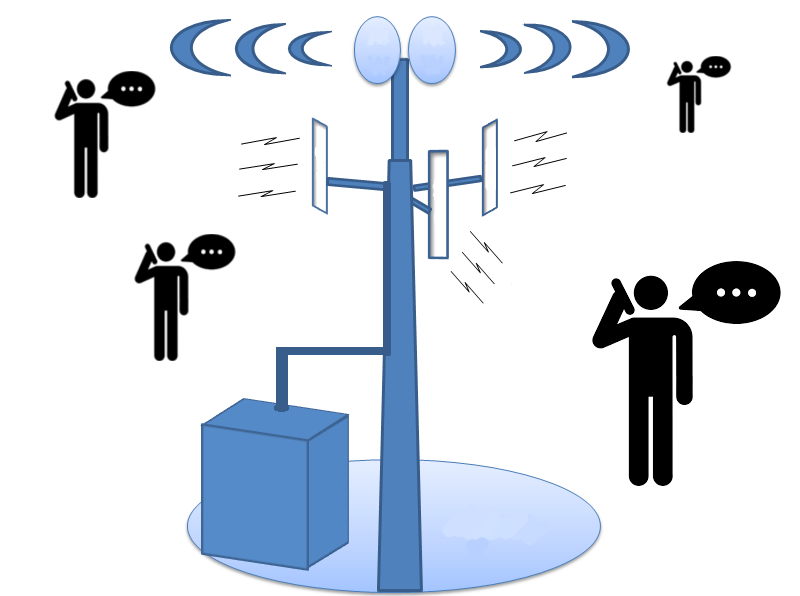
\includegraphics[scale=0.3]{btsppl.png}

\end{frame}


\begin{frame}{BBU/RRH}
  \centering
  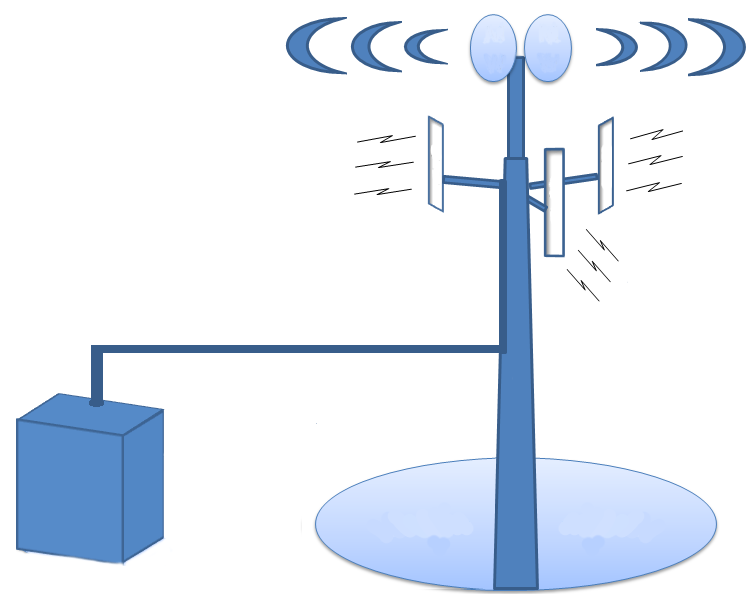
\includegraphics[scale=0.2]{cloudbts.png}\\
  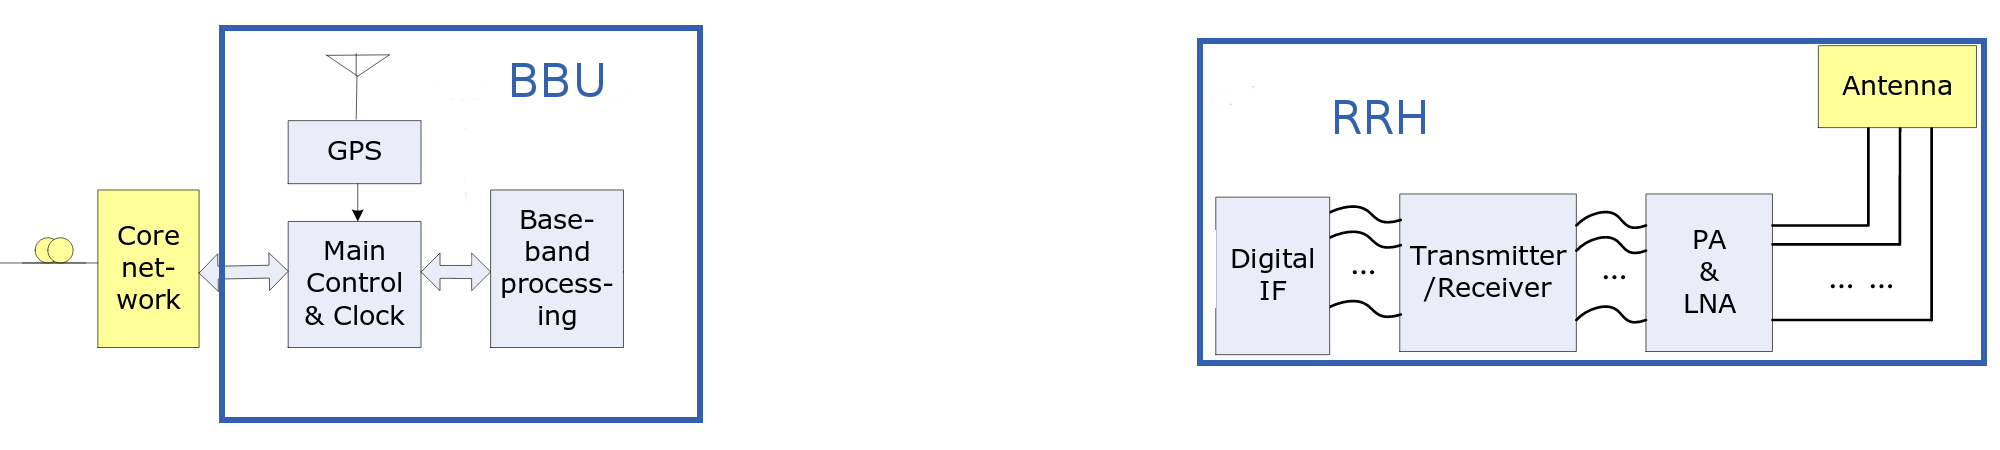
\includegraphics[scale=0.175]{BBURRH.png}
\end{frame}


\begin{frame}{Fronthaul}
  \centering
  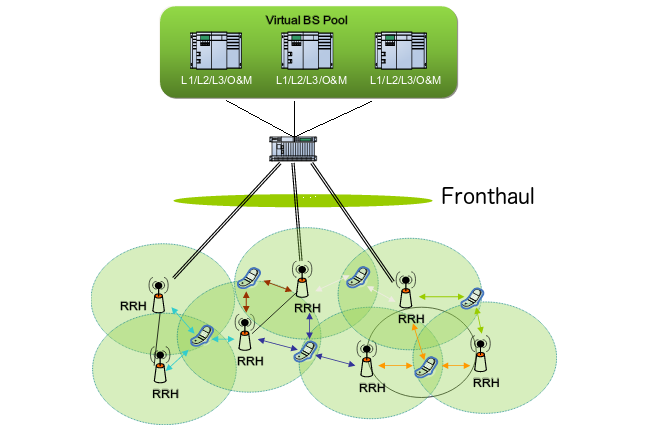
\includegraphics[scale=0.5]{CRAN}\\
  
\end{frame}

\begin{frame}{Problematic}
  \centering
  
  
 \begin{multicols}{2}
Constraints in Fronthaul network :
\vspace{1cm}
\begin{itemize}
\item Highly loaded
\item Periodic traffic
\item \textcolor{red}{Latency must be guaranteed}
\end{itemize}
\vspace{0.5cm}
Current approaches: \begin{itemize}
\vspace{1cm}
\item E2E connections $\rightarrow$ Too expensive
\item Statistical multiplexing $\rightarrow$ No latency guarantees  
\end{itemize}
\end{multicols}

\end{frame}



\begin{frame}{Model}

\centering
\scalebox{0.4}{

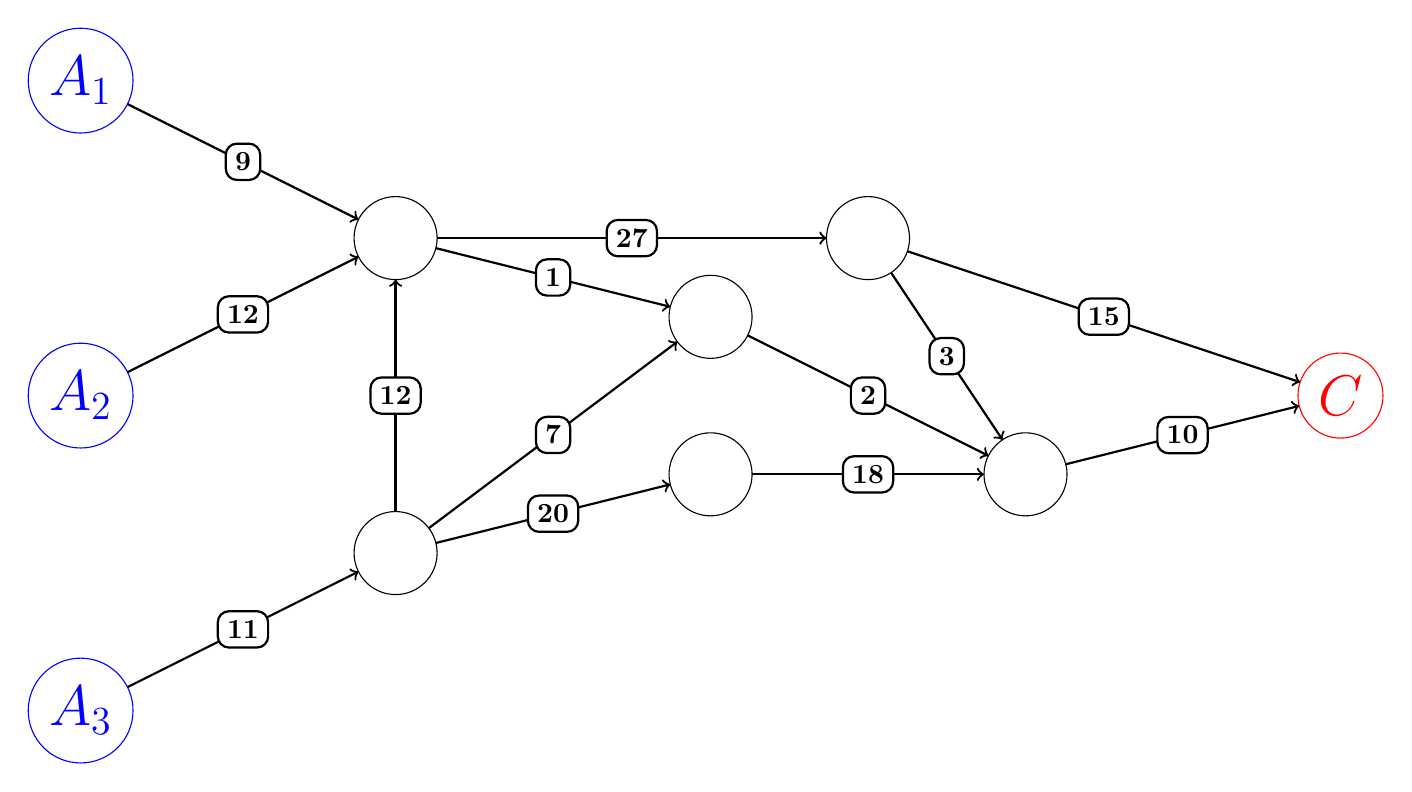
\begin{tikzpicture}
  \SetGraphUnit{5}
    \tikzset{
  EdgeStyle/.append style = {->} }
   \tikzstyle{VertexStyle}=[shape = circle, draw, minimum size = 30pt]
   \renewcommand{\VertexLightFillColor}{orange}
  \Vertex[x=0,y=0, L = {\huge $A_3$},style={blue}]{a3};
  \Vertex[x=0,y=4, L = {\huge $A_2$},style={blue}]{a2}
  \Vertex[x=0,y=8, L = {\huge $A_1$},style={blue}]{a1}


  \Vertex[x=16,y=4, L = {\huge $C$},style={red}]{c}
  
 \SetVertexNoLabel
  \Vertex[x=4,y=2]{n1}
  \Vertex[x=4,y=6]{n2}  
  \Vertex[x=12,y=3]{n4}
  \Vertex[x=8,y=3]{n6}
  \Vertex[x=8,y=5]{n7}
  \Vertex[x=10,y=6]{n8}



  \Edge[label = 12](n1)(n2)
  \Edge[label = 3](n8)(n4)
  \Edge[label = 15](n8)(c)
  \Edge[label = 27](n2)(n8)
  \Edge[label = 7](n1)(n7)
  \Edge[label = 9](a1)(n2)   
  \Edge[label = 2](n7)(n4)
  \Edge[label = 11](a3)(n1)
  \Edge[label = 20](n1)(n6)
  \Edge[label = 18](n6)(n4)
  \Edge[label = 12](a2)(n2)
  \Edge[label = 10](n4)(c)
  \Edge[label = 1](n2)(n7)

 
\end{tikzpicture}
}
\vspace{1cm}

 \end{frame}
  
 \begin{frame}{Collisions}

\begin{center}
\scalebox{0.4}{

\begin{tikzpicture}
  \SetGraphUnit{5}
    \tikzset{
  EdgeStyle/.append style = {->} }
   \tikzstyle{VertexStyle}=[shape = circle, draw, minimum size = 30pt]
   \renewcommand{\VertexLightFillColor}{orange}
  \Vertex[x=0,y=0, L = {\huge $a_3$}]{a3};
  \Vertex[x=0,y=4, L = {\huge $a_2$}]{a2}
  \Vertex[x=0,y=8, L = {\huge $a_1$}]{a1}


  \Vertex[x=16,y=4, L = {\huge $c$}]{c}
  
 \SetVertexNoLabel
  \Vertex[x=4,y=2]{n1}
  \Vertex[x=4,y=6]{n2}  
  \Vertex[x=12,y=3]{n4}
  \Vertex[x=8,y=3]{n6}
  \Vertex[x=8,y=5]{n7}
  \Vertex[x=10,y=6]{n8}



  \Edge(n1)(n2)
  \Edge(n8)(n4)
  \Edge(n8)(c)
  \Edge(n2)(n8)
  \Edge(n7)(n4)
  \Edge(n1)(n6)
  \Edge(n6)(n4)
  \Edge(a2)(n2)
  \Edge(n4)(c)

    
  \tikzset{
  EdgeStyle/.append style = {blue} }
  \Edge[label = 5](a1)(n2)   
   \Edge[label = 3](n2)(n7)
  
    \tikzset{
  EdgeStyle/.append style = {red} }
    \Edge[label = 2](a3)(n1)
      \Edge[label = 6](n1)(n7)
      
       \node (0) at (9,4){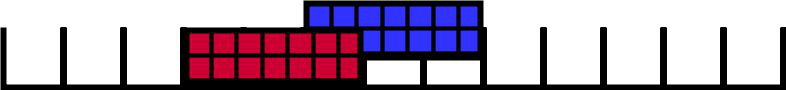
\includegraphics[scale=0.2]{col1.png}};


\end{tikzpicture}
}
\end{center}
\vspace{1cm}

\end{frame}

 \begin{frame}{Assignment }

\begin{center}
\scalebox{0.4}{

\begin{tikzpicture}
  \SetGraphUnit{5}
    \tikzset{
  EdgeStyle/.append style = {->} }
   \tikzstyle{VertexStyle}=[shape = circle, draw, minimum size = 30pt]
   \renewcommand{\VertexLightFillColor}{orange}
  \Vertex[x=0,y=0, L = {\huge $a_3$}]{a3};
  \Vertex[x=0,y=4, L = {\huge $a_2$}]{a2}
  \Vertex[x=0,y=8, L = {\huge $a_1$}]{a1}


  \Vertex[x=16,y=4, L = {\huge $c$}]{c}
  
 \SetVertexNoLabel
  \Vertex[x=4,y=2]{n1}
  \Vertex[x=4,y=6]{n2}  
  \Vertex[x=12,y=3]{n4}
  \Vertex[x=8,y=3]{n6}
  \Vertex[x=8,y=5]{n7}
  \Vertex[x=10,y=6]{n8}



  \Edge(n1)(n2)
  \Edge(n8)(n4)
  \Edge(n8)(c)
  \Edge(n2)(n8)
  \Edge(n7)(n4)
  \Edge(n1)(n6)
  \Edge(n6)(n4)
  \Edge(a2)(n2)
  \Edge(n4)(c)

    
  \tikzset{
  EdgeStyle/.append style = {blue} }
  \Edge[label = 5](a1)(n2)   
   \Edge[label = 3](n2)(n7)
  
    \tikzset{
  EdgeStyle/.append style = {red} }
    \Edge[label = 2](a3)(n1)
      \Edge[label = 6](n1)(n7)
      
       \node (0) at (9,4){
\includegraphics[scale=0.2]{col2.png}};


\end{tikzpicture}
}
\end{center}
\vspace{1cm}
\centering
Problem shown as NP-Hard and non-approximable
\end{frame}

\begin{frame}{Star network}
  \centering
\scalebox{0.4}{
\begin{tikzpicture}
    \SetGraphUnit{5}
  \tikzstyle{VertexStyle}=[shape = circle, draw, minimum size = 50pt]
  \Vertex[x=0,y=0]{a3}
  \Vertex[x=0,y=4]{a2}
  \Vertex[x=0,y=8]{a1}
  
  \Vertex[x=16,y=0]{c3}
  \Vertex[x=16,y=4]{c2}
  \Vertex[x=16,y=8]{c1}
  
  \SetVertexNoLabel
  \Vertex[x=4,y=4]{SL}
  \Vertex[x=12,y=4]{SS}  
  \tikzset{
  EdgeStyle/.append style = {<-,green} }
  \Edge(c1)(SS)
  \Edge(SL)(a1)
  
  \tikzset{
  EdgeStyle/.append style = {blue} }
  \Edge(c2)(SS)
  \Edge(SL)(a2)
  
  \tikzset{
  EdgeStyle/.append style = {red} }
  \Edge(c3)(SS)
  \Edge(SL)(a3)
  
  \tikzset{
  EdgeStyle/.append style = {black} }
  \Edge(SS)(SL)
  


\end{tikzpicture}
}

\centering
\vspace{1cm} One link shared by all routes.
\end{frame}



  
    \begin{frame}{Deterministic vs Stochastic}
\centering
\vspace{-2cm}
  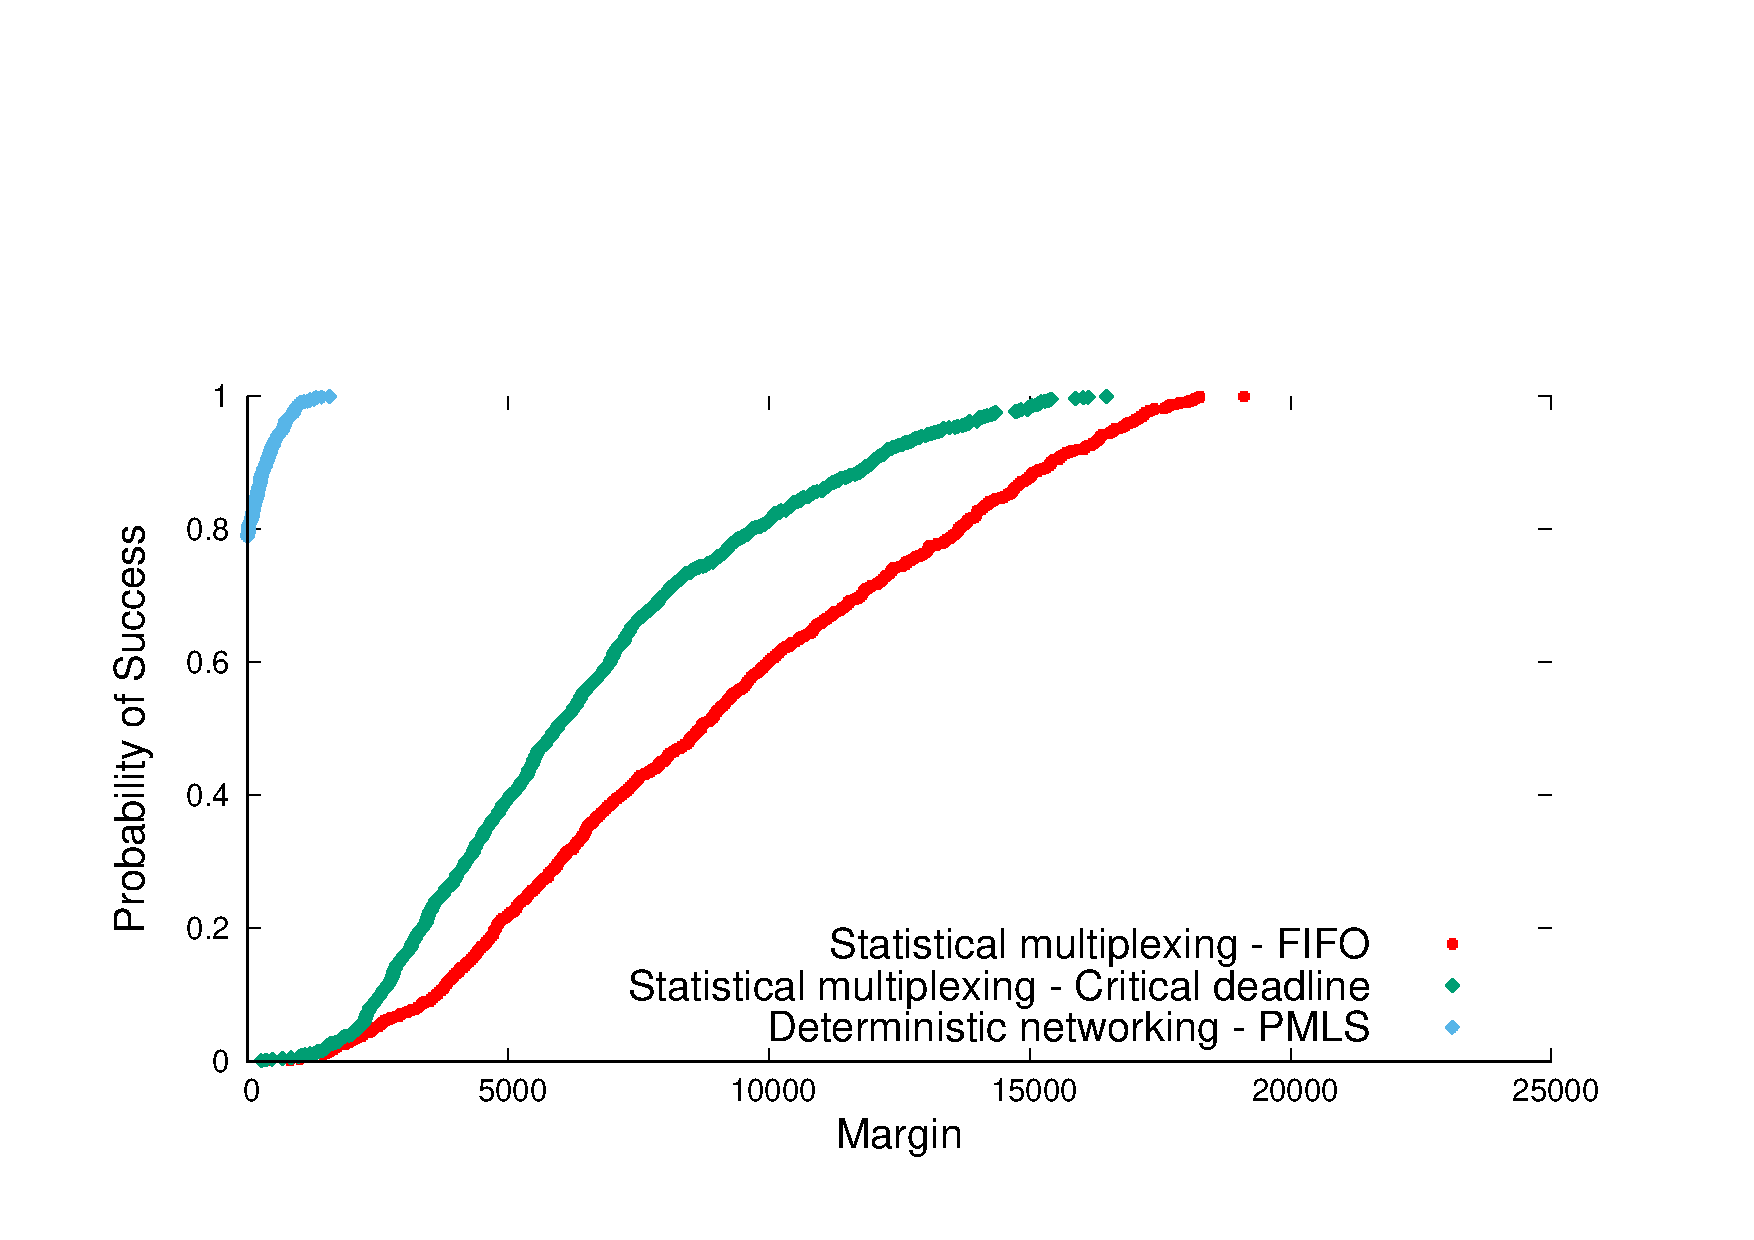
\includegraphics[scale=0.4]{stochastic.pdf}\\
  \end{frame}


\begin{frame}{More complex topology}
\centering
  \includegraphics[scale=0.8]{example23}\\

\end{frame}


\end{document}
